% !TEX encoding = UTF-8
% !TEX TS-program = pdflatex
% !TEX root = ../tesi.tex

% (3) che risponde alle domande “cosa” e “come”, nel quale racconterai gli elementi essenziali del tuo stage,
% vedendolo come un mini‐progetto a se stante. In questo capitolo illustrerai: (a) il metodo di lavoro con il quale hai
% affrontato lo stage; (b) i problemi progettuali, tecnologici e applicativi che hai affrontati; (c) i risultati che hai
% raggiunto, sia sul piano qualitativo che su quello quantitativo. Il punto (a) comprende la pianificazione, le interazioni
% con il tutor aziendale, le revisioni di progresso, l’uso di diagrammi, di tecniche di analisi e tracciamento dei requisiti,
% l’uso di strumenti di verifica, ecc. Il punto (b), che tratterai nella sequenza di attività che hai svolto (analisi,
% progettazione, programmazione, verifica e validazione), metterà in luce gli aspetti principali, secondo una visione ad
% alto livello. Entrerai in dettaglio solo per aspetti che consideri particolarmente meritevoli di attenzione dal punto di
% vista delle conoscenze acquisite o necessarie. Il punto (c) tratta di copertura di requisiti, di copertura di testing, e di
% quantità di prodotti (linee di codice, numero di documenti, ecc.).


%**************************************************************
\chapter{Resoconto dello stage}
\label{cap:resoconto-stage}
%**************************************************************

\section{Descrizione del progetto}
Il \textit{dataset} da elaborare ed analizzare è parte di un concorso a cui l'azienda aveva già partecipato qualche anno fa: questa competizione è stata indetta da BNP Paribas Cardif, il polo assicurativo del Gruppo BNP Paribas, e pubblicata su Keggle\footcite{https://www.kaggle.com/}, nota piattaforma in cui è possibile esporre i propri progetti, visualizzare quelli altrui e proporre sfide in ambito \textit{data science} e \textit{machine learning}.

\subsection{Il problema}
In particolare, il problema proposto, "BNP Paribas Cardif Claims Management"\footcite{https://www.kaggle.com/c/bnp-paribas-cardif-claims-management}, consiste nella possibilità di classificare le pratiche assicurative in modo che queste possano essere risolte nel minor tempo possibile. A tal proposito, si chiede di prevedere la categoria di un sinistro sulla base delle caratteristiche disponibili nelle prime fasi del processo assicurativo; le due categorie di richieste di indennizzo, su cui basare la classificazione, corrispondono quindi a:
\begin{itemize}
	\item Quelle per le quali l'approvazione può essere accelerata, con conseguente maggiore rapidità nel rimborso e minori pratiche da gestire;
	\item Quelle per le quali sono richieste informazioni supplementari prima dell'approvazione e del rimborso.
\end{itemize}
\clearpage
\begin{figure}[!h] 
	\centering 
	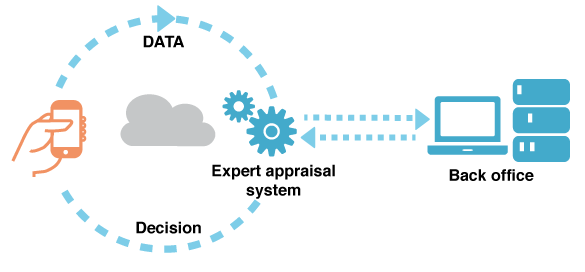
\includegraphics[width=0.6\columnwidth]{kaggle-project}
	\caption{Illustrazione del problema proposto (Fonte: \href{https://goo.gl/AW22at}{https://goo.gl/AW22at})}
\end{figure}
Nella sezione \hyperref[dataset]{Elaborazione del dataset di interesse} verrà trattata la struttura del \textit{dataset} più nel dettaglio.

%**************************************************************

\section{Studio di Hadoop e dei suoi tools}
Prima di cominciare a lavorare sul \textit{dataset} del progetto, era necessario studiare la teoria, in quanto la prima parte dello stage considerava argomenti a me quasi totalmente sconosciuti.
Autonomamente, ma sempre supervisionato dal tutor aziendale, disponibile a risolvere ogni mio dubbio, ho studiato il materiale necessario per poter eseguire poi al meglio la parte pratica. Oltre a ciò, nel corso della giornata lavorativa, il tutor mi sottoponeva delle esercitazioni da svolgere per consolidare i concetti appresi e risolvere tempestivamente miei eventuali dubbi prima di procedere con gli argomenti successivi.
Essendo \gls{HDFS} e molti dei tool Hadoop eseguibili principalmente tramite \gls{Bash}, come prima cosa il tutor mi ha assegnato lo studio autonomo di alcuni capitoli del libro "Learning the bash Shell"\footcite{http://shop.oreilly.com/product/9780596009656.do} per ottenere le basi che mi permettessero di utilizzare i comandi che avrei utilizzato in seguito per l'utilizzo dei tool Hadoop.\\
Dopo aver assorbito i concetti, già in parte di mia conoscenza, il tutor mi ha esposto la struttura del \gls{cluster} Hadoop in cui risiedevano i dati e venivano eseguiti i \textit{task}. 

\subsection{Apache Hadoop}
Ogni giorno si generano petabytes di dati che, se processati ed analizzati a dovere possono offrire informazioni con un alto valore strategico per un'azienda. Hadoop nasce dall'esigenza di dover gestire e processare questi dati in modo veloce, tramite una soluzione che sia il più possibile economica e scalabile orizzontalmente: aggiungendo nuovi nodi al \gls{cluster}, la capacità e le performance di questo infatti aumentano proporzionalmente. Per aumentare ulteriormente le prestazioni e la scalabilità del sistema, Hadoop cerca di elaborare i dati sullo stesso nodo in cui questi risiedono: questo permette di ridurre al minimo la \textit{cross-communication} fra i nodi e la necessità di copiare grandi quantità di dati fra questi, eliminando il rischio di \textit{bottleneck} dovuto dalla velocità di trasmissione dei dati. Per gestire il sistema, Hadoop si basa su:
\begin{itemize}
	\item \gls{HDFS}: per la gestione dei dati persistenti;
	\item YARN: per lo \textit{scheduling} dei processi (\textit{jobs}) e la gestione delle risorse.
\end{itemize}
\begin{figure}[!h]
	\centering 
	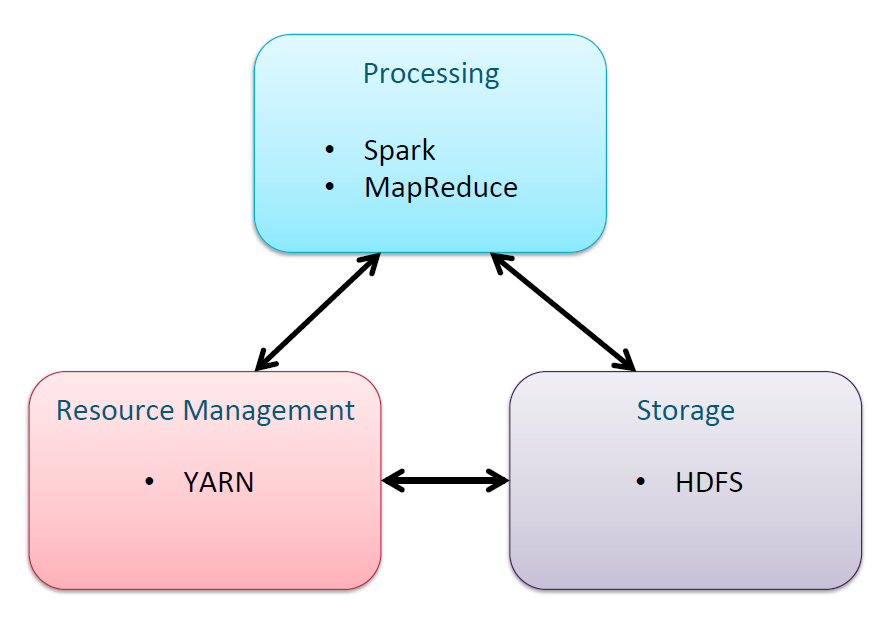
\includegraphics[width=0.7\columnwidth]{hadoop_tools}
	\caption{Attori principali del sistema Hadoop (Fonte: Cloudera - Developer Training for Spark and Hadoop)}
\end{figure}
\subsubsection{HDFS}
Hadoop Distributed File System (HDFS) è un \textit{file system} scritto in Java, basato su Google File System\footcite{https://ai.google/research/pubs/pub51}. \\
Offre performance migliori con un modesto numero di file di grandi dimensioni piuttosto che miliardi di file frammentati, per questo motivo, anche le operazioni di \textit{read}, sono ottimizzate per la lettura in \textit{streaming} piuttosto che quelle casuali. Inoltre, i file sono tutti \textit{write-once} e quindi non modificabili una volta memorizzati.
In scrittura, infatti, i dati sono suddivisi in blocchi di dimensione fissata e distribuiti tra i nodi in modo ridondante per prevenire la perdita di informazioni nel caso un nodo non fosse più disponibile in seguito.
\begin{figure}[!h]
	\centering
	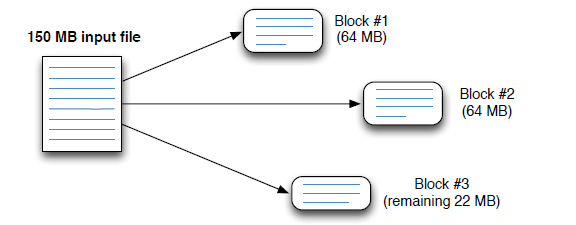
\includegraphics[width=0.8\columnwidth]{data_split}
	\caption{Divisione di un file in blocchi su HDFS (Fonte: Cloudera - Administrator Training for Apache Hadoop)}
\end{figure}
\clearpage
\begin{figure}[!h]
	\centering
	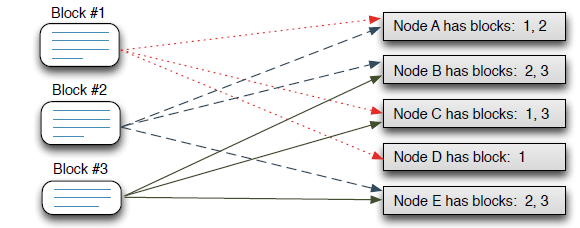
\includegraphics[width=0.8\columnwidth]{data_save}
	\caption{Caricamento dei blocchi nei nodi (Fonte: Cloudera - Administrator Training for Apache Hadoop)}
\end{figure}
Hadoop ha un'architettura di tipo \textit{master-slave}, ovvero in cui il processo \textit{master} ha il controllo su quello \textit{slave}. I nodi, quindi, possono essere di tre tipi:
\begin{itemize}
	\item \textbf{NameNode}: costituisce il \textit{master \gls{daemon}}, quindi gestisce tutti i metadati, le informazioni riguardo l'\textit{ownership} e i permessi ad una risorsa, i nomi dei blocchi e la loro locazione. Essendo unico e mantenendo la struttura del \textit{file system}, rappresenta un \gls{single point of failure} in \gls{HDFS};
	\item \textbf{DataNode}: costituisce gli \textit{slave \gls{daemon}}, quindi i nodi che contengono i blocchi di dati veri e propri;
	\item \textbf{Secondary NameNode}: esegue elaborazioni in supporto al NameNode. Non è un nodo di backup ma la funzione principale è quella di memorizzare una copia del file \textit{FsImage} e di modificare il file di log. \textit{FsImage} contiene un'istantanea dei metadati del \textit{file system} HDFS in un certo momento e \textit{EditLog} è il log delle transazioni che contiene record per ogni modifica dei metadati del \textit{file system}. In questo modo, in qualunque momento, è possibile ricostruire il NameNode a partire da \textit{FsImage} e applicando il record delle transazioni \textit{EditLog}.
\end{itemize}
\begin{figure}[!h]
	\centering
	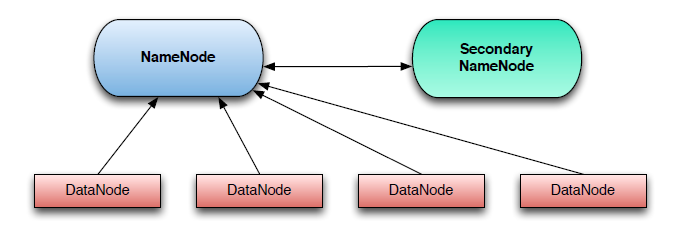
\includegraphics[width=0.8\columnwidth]{hadoop-nodes}
	\caption{Rappresentazione dei nodi in Hadoop (Fonte: Cloudera - Administrator Training for Apache Hadoop)}
\end{figure}
Nei seguenti esempi sono rappresentati semplici operazioni di scrittura e lettura sui nodi HDFS.
La procedura di scrittura di un blocco avviene nel seguente modo:
\begin{enumerate}
	\item Il client si connette al NameNode;
	\item NameNode registra i metadati del file e ritorna il nome del blocco e la lista dei DataNodes al client;
	\item Il client si connette al primo DataNode e comincia ad inviare i dati;
	\item A sua volta, il primo DataNode si connette al secondo e invia a sua volta i dati;
	\item Allo stesso modo, il secondo DataNode si connette al terzo;
	\item Ad ogni blocco scritto, al client viene ritornato un \textit{ack packets} dalla \textit{pipeline} di nodi;
	\item Una volta ricevuti tutti gli \textit{ack packets}, il client informa il NameNode del completamento della scrittura.
\end{enumerate} 
\begin{figure}[!h]
	\centering
	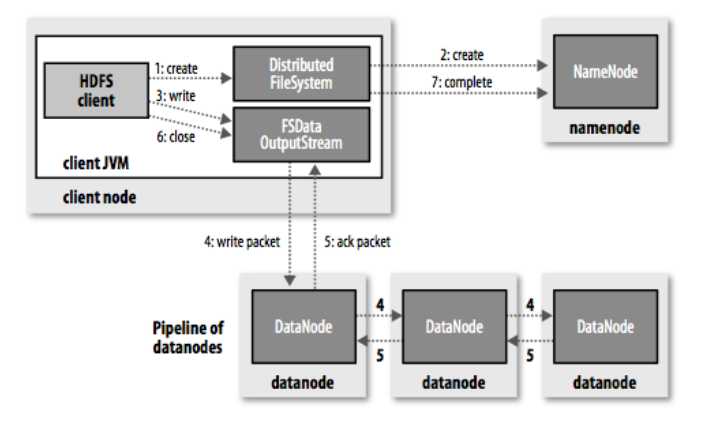
\includegraphics[width=0.65\columnwidth]{hdfs_write}
	\caption{Esempio di scrittura di un file in HDFS (Fonte: Cloudera - Administrator Training for Apache Hadoop)}
\end{figure}
La procedura di lettura di dati avviene nel seguente modo:
\begin{enumerate}
	\item Il client si connette al NameNode;
	\item NameNode ritorna il nome e la locazione dei blocchi del file;
	\item Il client si connette ai DataNodes comunicati e legge i blocchi.
\end{enumerate}
\begin{figure}[!h]
	\centering
	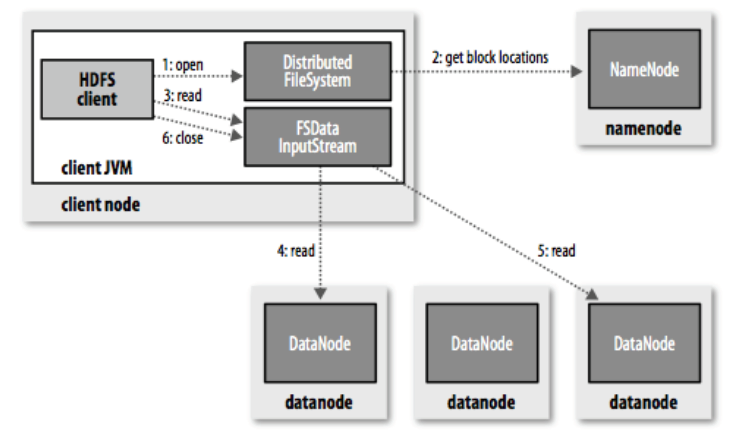
\includegraphics[width=0.65\columnwidth]{hdfs_read}
	\caption{Esempio di lettura di un file in HDFS (Fonte: Cloudera - Administrator Training for Apache Hadoop)}
\end{figure}

\subsubsection{YARN}
YARN (\textit{Yet Another Resource Negotiator}) è il manager delle risorse di Hadoop. I principali attori del sistema sono:
\begin{itemize}
	\item \textbf{ResourceManager}: uno per \gls{cluster}, e costituisce il \textit{master \gls{daemon}}; inizializza le applicazioni e ne pianifica l'utilizzo delle risorse sugli \textit{slave nodes}. È costituito da due componenti principali: uno \textit{scheduler} responsabile per l'allocazione delle risorse delle applicazioni al loro avvio ed un \textit{application manager} che gestisce le applicazioni già in esecuzione sul \textit{cluster};
	\item \textbf{NodeManager}: uno per \textit{slave nodes} e costituisce lo \textit{slave \gls{daemon}}; avvia i processi delle applicazioni e gestisce le risorse sul singolo \textit{slave node};
	\item \textbf{JobHistoryServer}: uno per \gls{cluster}, archivia i log ed i \textit{metadata} dei \textit{jobs} terminati;
	\item \textbf{ApplicationManager}: uno per applicazione, negozia le risorse con il ResourceManager e lavora con il NodeManager; gestisce l'intera vita dell'applicazione, dalla sua inizializzazione alla terminazione. 
\end{itemize}
\begin{figure}[!h]
	\centering
	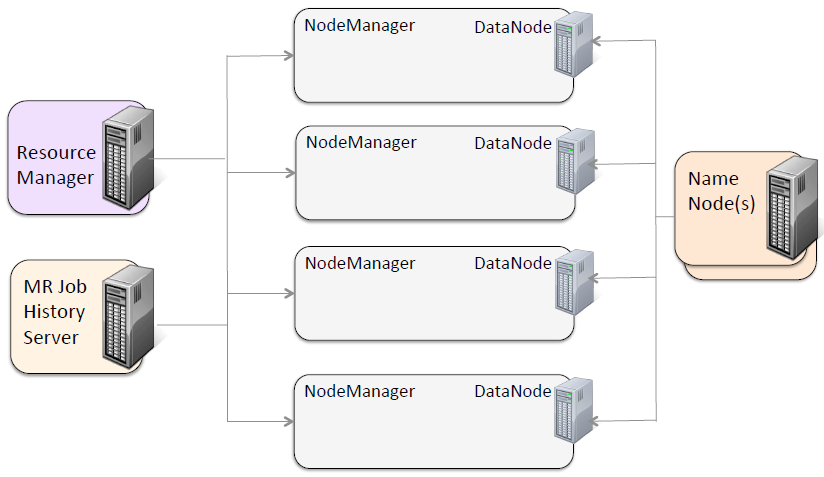
\includegraphics[width=0.8\columnwidth]{yarn_architecture}
	\caption{Struttura di un cluster che utilizza YARN (Fonte: Cloudera - Administrator Training for Apache Hadoop)}
\end{figure}
YARN, per avviare un'applicazione sul \gls{cluster}, si comporta nel modo seguente:
\begin{enumerate}
	\item Il client richiede di eseguire un \textit{job} al ResourceManager che inizializza un \textit{container}, ovvero un numero finito di risorse di un nodo, e avvia l'ApplicationManager sul NodeManager;
	\item L'ApplicationManager richiede le risorse necessarie per eseguire tutti i \textit{tasks} al ResourceManager;
	\item Il ResourceManager alloca nuovi \textit{containers} su altri nodi del \gls{cluster} e comunica all'ApplicationManager la loro locazione;
	\item L'ApplicationManager esegue i \textit{tasks} nei \textit{containers} allocati precedentemente;
	\item Una volta completato il \textit{job}, l'ApplicationManager segnala al ResourceManager la conclusione del processo.
\end{enumerate} 
\begin{figure}[!h]
	\centering
	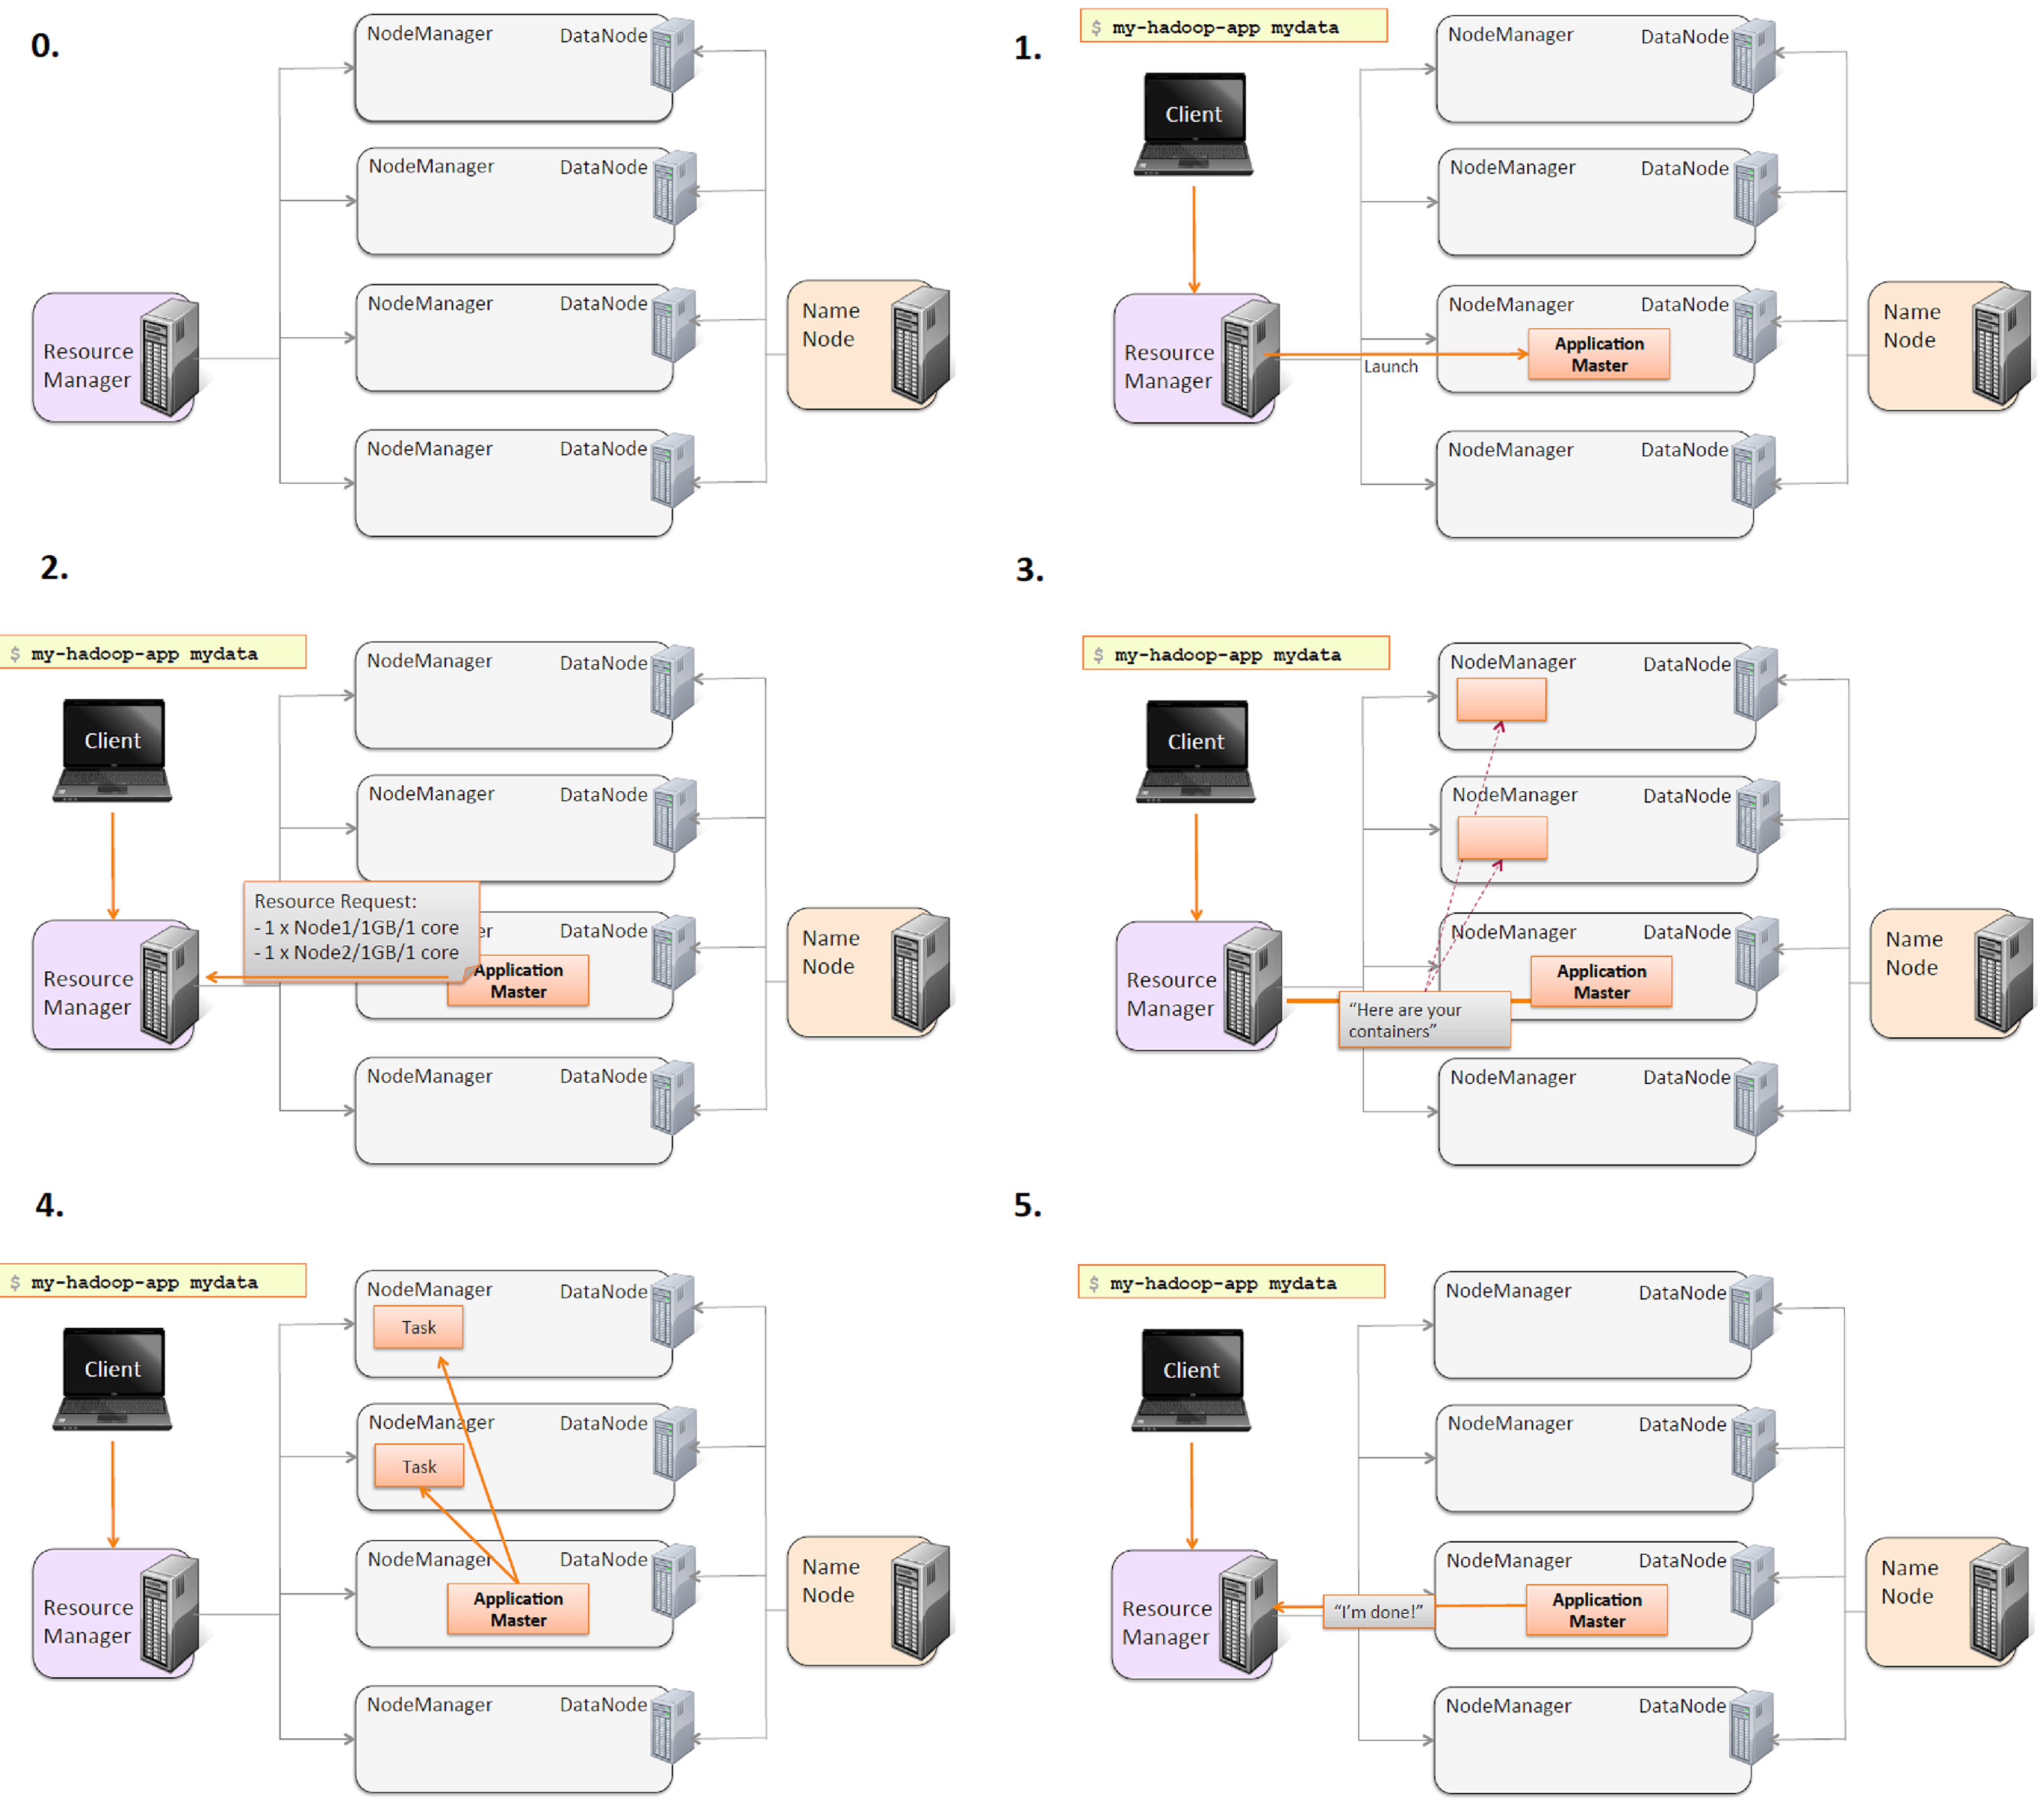
\includegraphics[width=1.1\columnwidth]{yarn_application}
	\caption{Sequenza avvio applicazione di YARN}
\end{figure}
\clearpage
\subsection{Apache Hive, Cloudera Impala e Apache Spark}
\subsubsection{Apache Hive}
Originariamente sviluppato da Facebook per facilitare le interrogazioni di \textit{dataset} su Hadoop, fornisce un metodo per effettuare \textit{query} in HDFS utilizzando un linguaggio simile ad SQL chiamato HiveQL. 
Le \textit{query} sono poi convertite da Hive in \textit{jobs} che vengono eseguiti da YARN. A causa di questa conversione, i risultati di una \textit{query} sono lenti, infatti ottenere un risultato può richiedere anche minuti se non ore. Inoltre, come detto in precedenza, in HDFS non è possibile modificare i dati, e quindi le operazioni di UPDATE e DELETE, tipiche di SQL, non sono supportate.\\
Hive interpreta tutti i file di una directory HDFS come contenuti di una tabella e salva le informazioni su come le righe e le colonne della tabella sono delimitate in una locazione, che può essere sulla macchina locale dell'utente o condivisa fra più utenti, chiamata \textbf{Hive Metastore}.
\begin{figure}[!h]
	\centering
	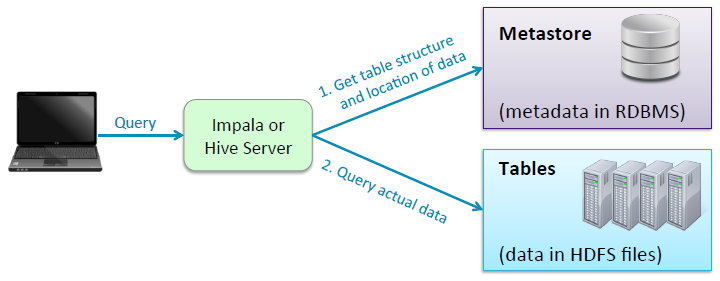
\includegraphics[width=0.8\columnwidth]{query}
	\caption{Esecuzione di una query (Fonte: Cloudera - Data Analyst Training)}
\end{figure}
\\Nel caso Hive Metastore sia condiviso, il client si connette ad un altro attore, chiamato \textbf{Hive Metastore Service} utilizzando le \gls{api} di Apache Thrift\footcite{https://thrift.apache.org/}. A sua volta, questo si connette al Metastore attraverso \gls{Java JDBC}.
\begin{figure}[!h]
	\centering
	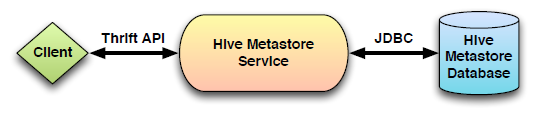
\includegraphics[width=0.8\columnwidth]{hive-metastore}
	\caption{Rappresentazione delle connessioni ad Hive Metastore (Fonte: Cloudera - Administrator Training for Apache Hadoop)}
\end{figure}

\subsubsection{Cloudera Impala}
Impala è derivato da Hive e, come quest'ultimo, permette di effettuare \textit{query} su HDFS utilizzando HiveQL. Inoltre, eredita l'utilizzo dello stesso Metastore condiviso per i metadati delle tabelle ma, a differenza di Hive, non converte le \textit{query} in \textit{jobs}. Infatti le \textit{query} di Impala vengono eseguite su un ulteriore insieme di \gls{daemon}, indicati come \textbf{Impala Servers}, sul \gls{cluster} Hadoop. Questo permette ad Impala di eseguire \textit{query} molto più velocemente di Hive ma, in contrapposizione, non supporta tutti i tipi complessi e le operazioni di Hive.\\
Gli Impala Servers risiedono su ogni DataNode dell'applicazione, mentre \textbf{Impala State Store Server} e \textbf{Impala Catalog Server}, che hanno lo scopo di gestire gli Impala Servers, sono unici nel \gls{cluster} e sono tipicamente locati sul NameNode. 
\begin{figure}[!h]
	\centering
	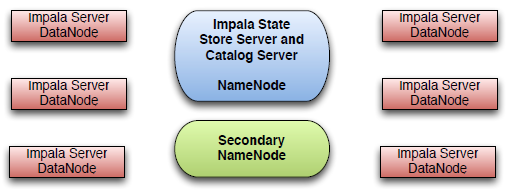
\includegraphics[width=0.8\columnwidth]{impala-servers}
	\caption{Rappresentazione dei daemons Impala (Fonte: Cloudera - Administrator Training for Apache Hadoop)}
\end{figure}

\begin{figure}[!h]
	\centering
	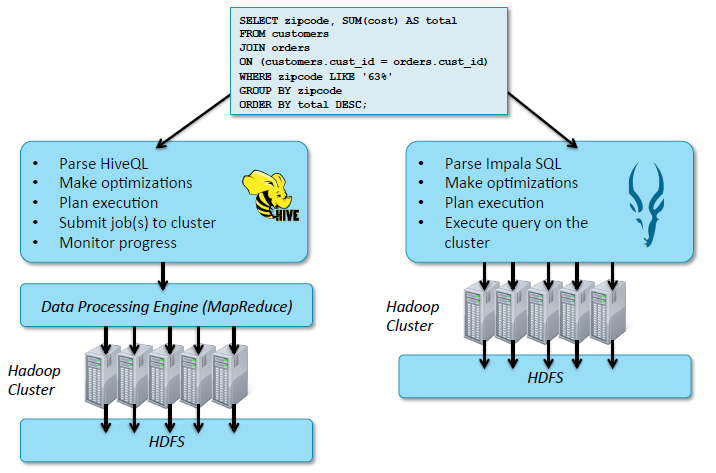
\includegraphics[width=1\columnwidth]{hive-impala}
	\caption{Differenza tra l'esecuzione di query in Hive ed Impala (Fonte: - Administrator Training for Apache Hadoop)}
\end{figure}

\subsubsection{Apache Spark}
Spark è un \textit{framework} scritto in Scala\footcite{https://www.scala-lang.org/} per il \textit{processing} dei dati in \textit{dataset} di grandi dimensioni.
È possibile eseguire attività di Spark tramite la \gls{Bash} o tramite applicazioni scritte in linguaggio Python, Scala o Java e poi eseguite su Hadoop.
La maggior parte delle operazioni vengono eseguite tramite l'utilizzo di \textbf{RDD} (Resilient Distributed Dataset), che sono la rappresentazione più semplice dei dati in Spark e sono immutabili. Su di un RDD sono possibili due tipi di operazioni:
\begin{itemize}
	\item \textbf{Actions}: semplici attività terminali che restituiscono un valore, come \textit{count}, \textit{take} o \textit{collect}; 
	\item \textbf{Transformations}: tramite le quali viene creato un nuovo RDD partendo da quello su cui è invocata l'operazione. Questo tipo di attività è necessario se si vuole modificare l'RDD di partenza, essendo questo immutabile. Operazioni tipiche sono \textit{map} e \textit{filter}.
\end{itemize}
\begin{figure}[!h]
	\centering
	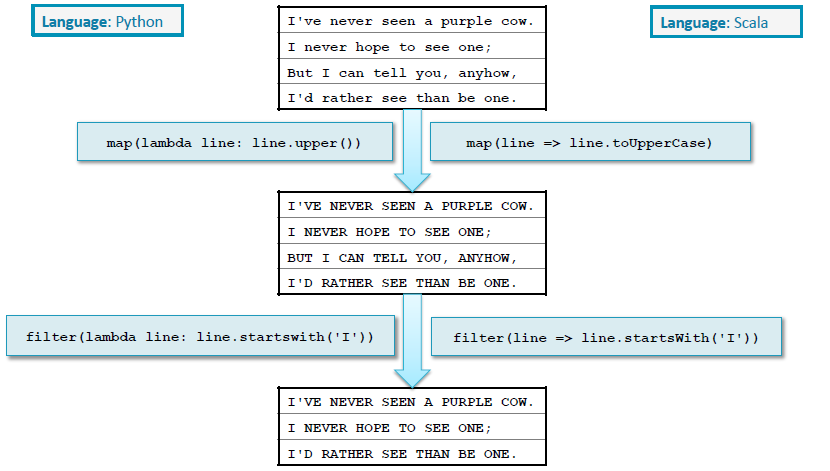
\includegraphics[width=1\columnwidth]{spark-op}
	\caption{Esempio di operazioni in Spark}
\end{figure}
L'esecuzione delle attività negli RDD è \textit{lazy}, ovvero la \textit{pipeline} di operazioni non viene eseguita finché non incontra un'operazione terminale data da una \textit{action}. Inoltre, durante l'esecuzione della \textit{pipeline} delle operazioni, non viene salvato alcun risultato intermedio finché non viene eseguita un'operazione terminale.\\\\
Un altro tipo di struttura dati, oltre ad RDD, supportata da Spark sono i \textbf{DataFrame}: questi sono \textit{dataset} organizzati con uno schema e quindi con colonne nominali. Come risultato si ottengono delle tabelle simili a quelle di un database relazionale ma con ulteriori ottimizzazioni per rendere le operazioni su di questi molto più veloci. Per eseguire queste operazioni, Spark mette a disposizione Spark SQL, un modulo per il \textit{processing} dei dati strutturato, basato sul linguaggio SQL.
%**************************************************************
\newpage
\section{Elaborazione del dataset di interesse} \label{dataset}
Il dataset oggetto del concorso\footcite{https://www.kaggle.com/c/bnp-paribas-cardif-claims-management/data} è composto da due parti:
\begin{itemize}
	\item "train.csv": che contiene i dati su cui effettuare le analisi e su cui basare il modello statistico;
	\item "test.csv": che contiene i dati su cui verranno testati i modelli stimati dai partecipanti, ed in base a cui si dichiarerà il vincitore del concorso.
\end{itemize}
Il \textit{dataset} è anonimo, in quanto contiene dati sensibili provenienti da clienti di BNP Paribas Cardif, e contiene dati sia di tipo categoriale che numerico.  È composto da 132 colonne e 114321 righe a cui si aggiunge una colonna, "target", per il \textit{dataset} train, che contiene il risultato su cui stimare il modello. Oltre alla colonna "ID", che identifica in modo univoco l'ennupla, non si ha alcun altra informazione sui valori.\\\\
Per effettuare le operazioni sul \textit{dataset}, che al momento del mio utilizzo era già presente nel \gls{cluster} dell'azienda, è stato utilizzato solamente Spark. Nello specifico, ho utilizzato il linguaggio Scala per scrivere la \textit{pipeline} di operazioni da eseguire sul \gls{cluster}. È stato possibile utilizzare solamente Spark e non Hive o Impala in quanto, utilizzando i DataFrame come spiegato nella sezione precedente, è possibile utilizzare Spark SQL per effettuare le \textit{query} sui dati in modo semplice con un linguaggio simile ad SQL.
Questo mi ha permesso di concentrarmi solamente sulla scrittura della pipeline di operazioni in Scala, da cui poi si è ricavato il \gls{JAR} eseguito sul \gls{cluster}.
Le operazioni di elaborazione del \textit{dataset} richieste sono:
\begin{enumerate}
	\item Identificazione del tipo (intero, double o stringa) della colonna e calcolo di statistiche di interesse sui valori contenuti;
	\item Calcolo della matrice di correlazione fra le varie colonne del \textit{dataset}.
\end{enumerate}
Tutte le operazioni sui dati sono state effettuate sul \textit{dataset} "train.csv" in quanto soggetto per la stima del modello.

\subsection{Identificazione tipo e calcolo dati statistici}
Per quanto riguarda il primo punto, identificare il tipo delle colonne, ho preventivamente escluso i valori vuoti o nulli.
In seguito, ho valutato i valori rimanenti: le colonne contenenti dati di tipo stringa sono state considerate come categoriali, mentre le rimanenti come numeriche. 
Dopo aver identificato le colonne, in base al tipo di queste,ho valutato i valori e calcolato le statistiche di interesse:
\begin{itemize}
	\item Per le colonne di tipo categoriale, il progetto richiedeva l'identificazione dei valori univoci ed il calcolo delle relative occorrenze;
	\item Per le colonne di tipo numerico, il progetto richiedeva il valore minimo, massimo, medio e la deviazione standard dei valori presenti.
\end{itemize}
Per entrambi i tipi, inoltre, il progetto richiedeva il conteggio delle righe vuote per ogni colonna, così da identificare eventuali variabili che, se non significative, sarebbero state scartate durante l'analisi.
\clearpage
\begin{figure}[!h]
	\centering
	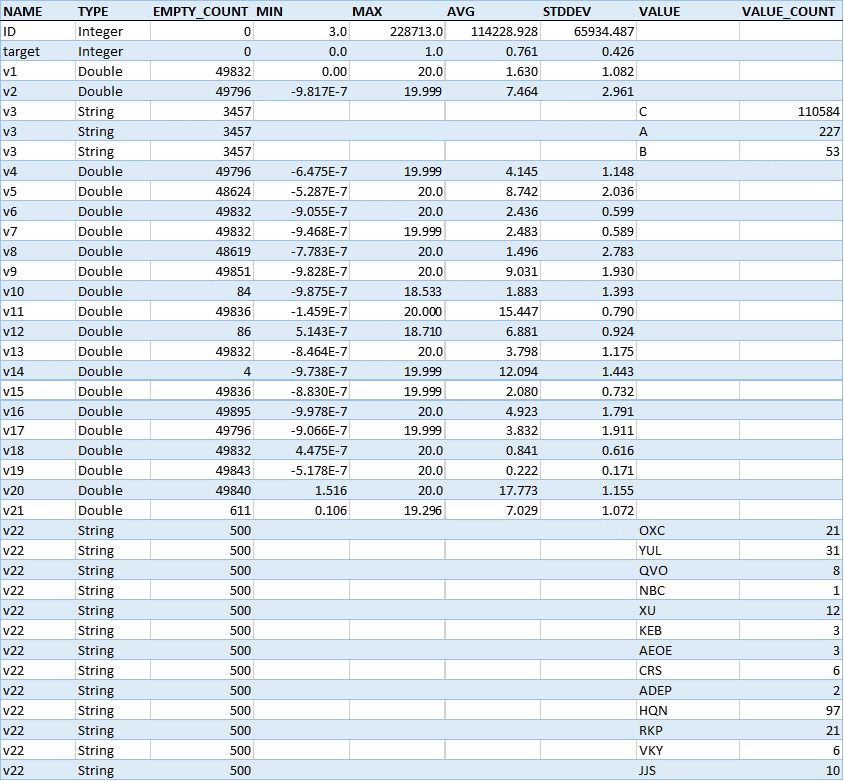
\includegraphics[width=1\columnwidth]{stats}
	\caption{Esempio del CSV contenente le statistiche delle variabili ottenute}
\end{figure}

\subsection{Calcolo della matrice di correlazione}
La matrice di correlazione è un indice che esprime un'eventuale relazione di linearità tra le variabili su cui è calcolato. Si rivela dunque molto utile per la stima del modello statistico, in quanto si dimostra un'analisi preliminare valida per una prima stima delle variabili significative per il modello.\\
Nel caso particolare di questo progetto, ho costruito la matrice di correlazione utilizzando tutte e 133 le variabili. La colonna le cui correlazioni sono più interessanti è ovviamente la variabile "target", ma anche le correlazioni tra le altre colonne sono di interesse per capire se ci sono interazioni tra loro. Per questo motivo, tramite Spark, mi sono limitato a costruire la matrice di correlazione completa e poi, nella \gls{web app} sviluppata, ho implementato la possibilità di visionare la matrice completa o solamente contenente le relazioni tra le variabili e "target".

\begin{figure}[!h]
	\centering
	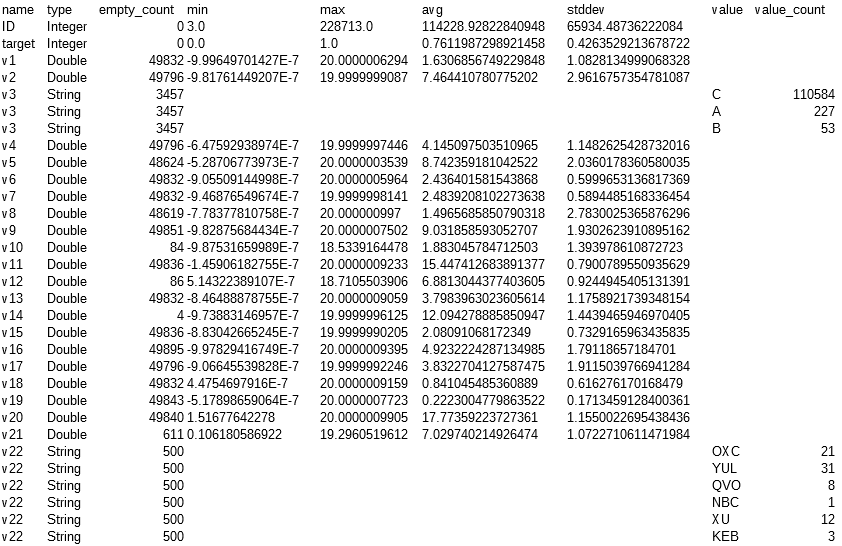
\includegraphics[width=1\columnwidth]{corr}
	\caption{Esempio del CSV contenente la matrice di correlazione tra variabili}
\end{figure}

Una volta concluse queste elaborazioni, ho mostrato il lavoro svolto al tutor che mi ha seguito per la parte \textit{big data} e, dopo essermi confrontato su quanto ottenuto e su cosa visualizzare nella \gls{web app} che avrei realizzato a breve, ha validato la conclusione della parte di lavoro di elaborazione del \textit{dataset}.

%**************************************************************
\clearpage
\section{Progettazione e sviluppo della web app}
A seguito delle elaborazioni effettuate, mi ha affiancato un nuovo tutor, facente parte del reparto di sviluppo software. Come da \hyperref[pdl]{Piano di Lavoro}, nella seconda parte del periodo di stage era programmato il ripasso di Java con attenzione all'ambiente Java EE. Per fare ciò, mi sono documentato soprattutto tramite la documentazione ed i tutorial ufficiali\footcite{https://docs.oracle.com/javaee/7/tutorial/index.html} forniti da Oracle. Rispetto alla prima parte di stage, relativa ai \textit{big data}, lo studio e lo svolgimento di esercizi riepilogativi che mi permettessero di mettere in pratica le conoscenze acquisite è stato più autonomo. Questo perchè, essendo alcune conoscenze di Java e sullo sviluppo di \gls{web app} già in mio possesso, non ho incontrato particolari difficoltà, se non alcuni dubbi che il tutor ha risolto tempestivamente.
Per quanto riguarda la scelta dello strumento per sviluppare la parte di \textit{front-end}, inizialmente ho optato per le librerie React e Redux, in quanto già di mia conoscenza. Confrontandomi con il tutor, però, sono arrivato alla conclusione che l'utilizzo di Angular sarebbe stata la miglior scelta: in questo modo avrei potuto sfruttare il periodo in azienda per acquisire queste nuove conoscenze affiancato da personale qualificato ed esperto che avrebbe potuto aiutarmi in caso di incertezze. \\
I requisiti individuati per la \gls{web app} seguono questa convenzione:\\\\
\centerline{\textbf{R[Tipo][Importanza][Codice]}}\\
Dove:
\begin{itemize}
	\item \textbf{Tipo}: specifica la tipologia del requisito e può assumere i valori:
	\subitem - F: requisito funzionale;
	\subitem - V: requisito di vincolo.
	\item \textbf{Importanza}: specifica l'importanza del requisito e può assumere i valori:
	\subitem - O: requisito obbligatorio;
	\subitem - D: requisito desiderabile;
	\subitem - P: requisito opzionale; 
	\item  \textbf{Codice}: è il codice gerarchico univoco di ogni requisito espresso in numeri.
\end{itemize} 
\clearpage
\begin{table}[!h] %
	\caption{Requisiti per la web app}
	\label{tab:requisiti-app}
	\centering
	\begin{tabular}{ l | l }
		\textbf{Codice} & \textbf{Descrizione}\\
		\hline
		\hline
		\\[-2.5mm]
		RFO01 & L'utente deve poter visualizzare le statistiche delle variabili \\
		\hline
		\\[-2.5mm]
		RFO02 & L'utente deve poter visualizzare la matrice di correlazione completa \\
		\hline
		\\[-2.5mm]
		RFO03 & L'utente deve poter visualizzare la correlazione fra "target" e le altre \\ & variabili \\
		\hline
		\\[-2.5mm]
		RFO04 & L'utente deve poter effettuare la ricerca di una specifica variabile \\
		\hline
		\hline
		\\[-2.5mm]
		RFD01 & L'utente deve poter visualizzare dei grafici statistici per le variabili \\ & numeriche \\
		\hline
		\\[-2.5mm]
		RFD02 & L'utente deve poter visualizzare dei grafici statistici per le variabili \\ & categoriali \\
		\hline
		\\[-2.5mm]
		RFD03 & L'utente deve poter visualizzare le tre maggiori correlazioni di una \\ 
		& variabile \\
		\hline
		\\[-2.5mm]
		RFD04 & L'utente deve poter impostare un limite inferiore della correlazione tra \\ & "target" e le altre variabili \\
		\hline
		\hline
		\\[-2.5mm]
		RVO01 & Utilizzo di Java EE \\
		\hline
		\hline
		\\[-2.5mm]
		RVD01 & Sviluppo di un'architettura three-tier \\
		\hline
		\end{tabular}
\end{table}%
Inoltre, ho concordato assieme al tutor di utilizzare le risorse create a seguito dell' \hyperref[dataseta]{elaborazione del \textit{dataset}} salvate in locale e non sul \gls{cluster}, in quanto l'amministratore di sistema, durante il mio ultimo periodo di stage, era impossibilitato a configurare l'accesso ad Hadoop tramite \gls{Java JDBC}. \\
Data la natura didattica e la relativa semplicità della \gls{web app}, dopo il consiglio del tutor aziendale, ho scelto di utilizzare GlassFish\footcite{https://javaee.github.io/glassfish/} come \textit{application server} in quanto ben supportato.
Prima di cominciare con la progettazione del prodotto, ho inoltre considerato le operazioni necessarie sui dati da presentare già in possesso: era infatti richiesta la sola lettura di questi, quindi non mi sono preoccupato di impostare un sistema che fosse in grado di dare la possibilità all'utente di modificare i dati, essendo questa operazione non necessaria per la \gls{web app}.

\subsection{Architettura software}
Come architettura del software, ho scelto una semplice architettura \textit{three-tier}, che si compone di tre elementi principali:
\begin{itemize}
	\item \textbf{Presentation tier}: (primo livello) responsabile della presentazione e dell'interazione con l'utente; 
	\item \textbf{Business Logic tier}: (secondo livello) i processi in questo livello gestiscono la logica dell'applicazione. Si frappongono fra il primo ed il terzo livello, cosicchè il client (primo livello) non comunicherà mai direttamente con i dati persistenti del livello inferiore; in questo modo, in questo strato, è possibile elaborare i dati e gestire la sicurezza prima dell'accesso alla risorsa persistente;
	\item \textbf{Data tier}: (terzo livello) contiene i dati salvati in un database o in un \textit{filesystem}; questi dati possono essere acceduti solamente dal livello superiore.
\end{itemize}

\begin{figure}[!h]
	\centering
	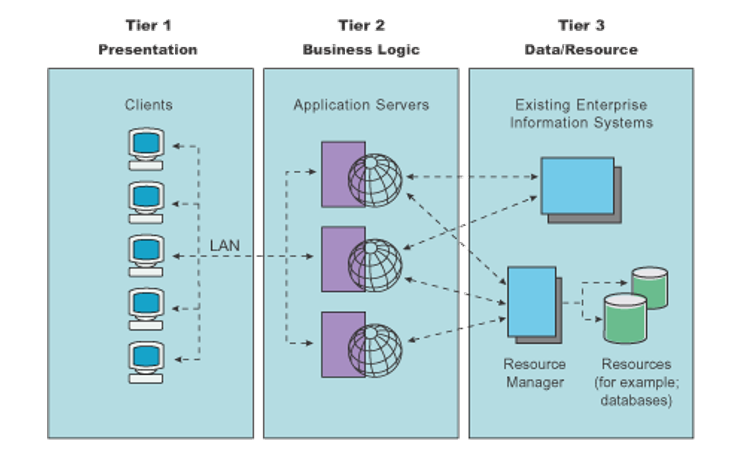
\includegraphics[width=0.8\columnwidth]{3-tier}
	\caption{Esempio di architettura three-tier generica (Fonte: \href{https://goo.gl/nuFksu}{https://goo.gl/nuFksu})}
\end{figure}

Nella figura sottostante è possibile vedere come sia applicata un'architettura \textit{three-tier} in ambiente Java EE.
\begin{figure}[!h]
	\centering
	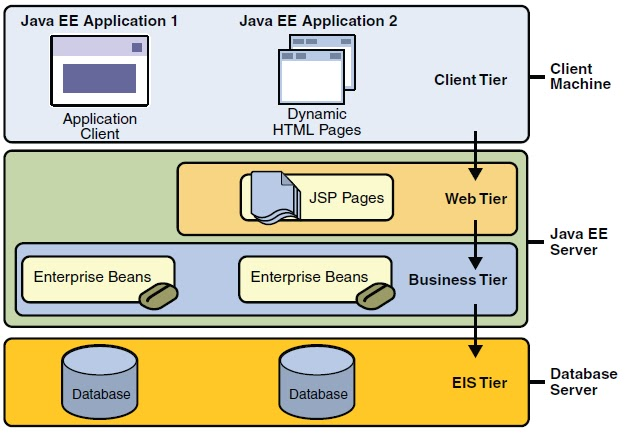
\includegraphics[width=0.8\columnwidth]{3-tier_java}
	\caption{Esempio di architettura three-tier in Java EE (Fonte: \href{https://goo.gl/S6RYgT}{https://goo.gl/S6RYgT})}
\end{figure}

Per lo sviluppo del prodotto, ho deciso di utilizzare un insieme di tecnologie offerte da Java EE.
\subsubsection{JavaServer Pages}
Le JavaServer Pages (JSP) permettono di sviluppare pagine web generate dinamicamente, innestando codice Java all'interno di semplici pagine HTML. Per eseguire il codice Java e generare i contenuti dinamici, questo viene eseguito a \textit{runtime} e trasformato in servlet dal server in cui la \gls{web app} è in esecuzione e poi il risultato elaborato viene restituito al client.
Nel mio caso ho sviluppato tre JSP:
\begin{itemize}
	\item corrMatrix.jsp: contenente la pagina di visualizzazione della matrice di correlazione;
	\item corrTarget.jsp: contenente la pagina di visualizzazione delle correlazioni fra "target" e le altra variabili;
	\item listData.jsp: contenente le statiche delle variabili.
\end{itemize}
\subsubsection{Java Servlet}
I servlet sono oggetti che operano all'interno di un server web (es. Tomcat) oppure un server per applicazioni (come nel mio caso, GlassFish) permettendo la creazione di applicazione web e l'elaborazione di richieste da parte di un client.
I servlet sono associati ad uno specifico \textit{URL} a seconda dei parametri di richiesta inviati dal client browser dell'utente al server e, una volta invocati, sono responsabili della pagina da visualizzare o quale parte dell'applicazione invocare.\\
Il flusso di dati di un servlet avviene nel seguente modo:
\begin{enumerate}
	\item Un client invia una richiesta (\textit{request}) per un servlet ad un server;
	\item Qualora si tratti della prima richiesta, il server istanzia e carica il servlet in questione avviando un \textit{thread} che gestisca la comunicazione con il servlet stesso. Nel caso, invece, in cui il servlet sia già stato caricato in precedenza allora verrà, più semplicemente, creato un ulteriore \textit{thread} che sarà associato al nuovo client, senza la necessità di ricaricare ancora il servlet;
	\item Il server invia al servlet la richiesta pervenutagli dal client;
	\item Il servlet costruisce ed imposta la risposta (\textit{response}) e la inoltra al server;
	\item Il server invia la risposta al client.
\end{enumerate}
\begin{figure}[!h]
	\centering
	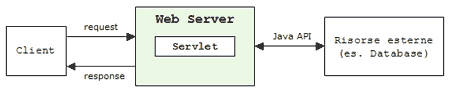
\includegraphics[width=0.8\columnwidth]{flusso-servlet}
	\caption{Flusso di dati in un servlet}
\end{figure}

Nel mio caso ho sviluppato i seguenti servlet:
\begin{itemize}
	\item DataServlet.java: contenente il servlet per l'inizializzazione  dei contenuti di listData.jsp e dei relativi dati;
	\item MatrixServlet.java: contenente il servlet per l'inizializzazione  dei contenuti di corrMatrix.jsp e dei relativi dati;
	\item TargetServlet.java: contenente il servlet per l'inizializzazione  dei contenuti di corrTarget.jsp e dei relativi dati;
	\item UtilCorrServlet.java: risponde inviando oggetti di tipo \gls{JSON} alle richieste di dati da parte degli script Angular per la visualizzazione dei grafici relativi alla correlazione fra "target" e le altre variabili;
	\item UtilStatsServlet.java: risponde inviando oggetti di tipo \gls{JSON} alle richieste di dati da parte degli script Angular per la paginazione dei risultati e la visualizzazione dei grafici relativi alle statistiche delle variabili.
\end{itemize}

\subsubsection{Enterprise JavaBeans}
Gli Enterprise JavaBeans (EJB) sono i componenti software che implementano, lato server, la logica di business di una \gls{web app} all'interno della piattaforma Java EE, per definire il contenuto dinamico da mostrare al client, che può essere una pagina JSP, un servlet o anche un altro EJB o una classe generica Java. Risiedono dunque su un \textit{application server} e sono tipicamente utilizzati in architetture software di tipo \textit{multi-tier}.
Nel mio caso ho sviluppato tre beans:
\begin{itemize}
	\item Data.java: contenente il modello dei dati delle variabili e delle relative statistiche;
	\item Matrix.java: contenente il modello dei dati della matrice di correlazione;
	\item Target.java: contenente il modello dei dati delle correlazioni fra "target" e le altre variabili;
\end{itemize}

Oltre a queste classi, contenenti i modelli base degli oggetti, ho sviluppato altre tre classi per gestire alcuni metodi statici di servizio per semplificare il modello dei beans, ad esempio per la lettura dei dati dai file \gls{CSV}.\\\\
La composizione di questi tre componenti offerti da Java EE permette di ottenere un'architettura \textit{three-tier} che implementa il pattern architetturale MVC (Model-View-Controller).
\begin{figure}[!h]
	\centering
	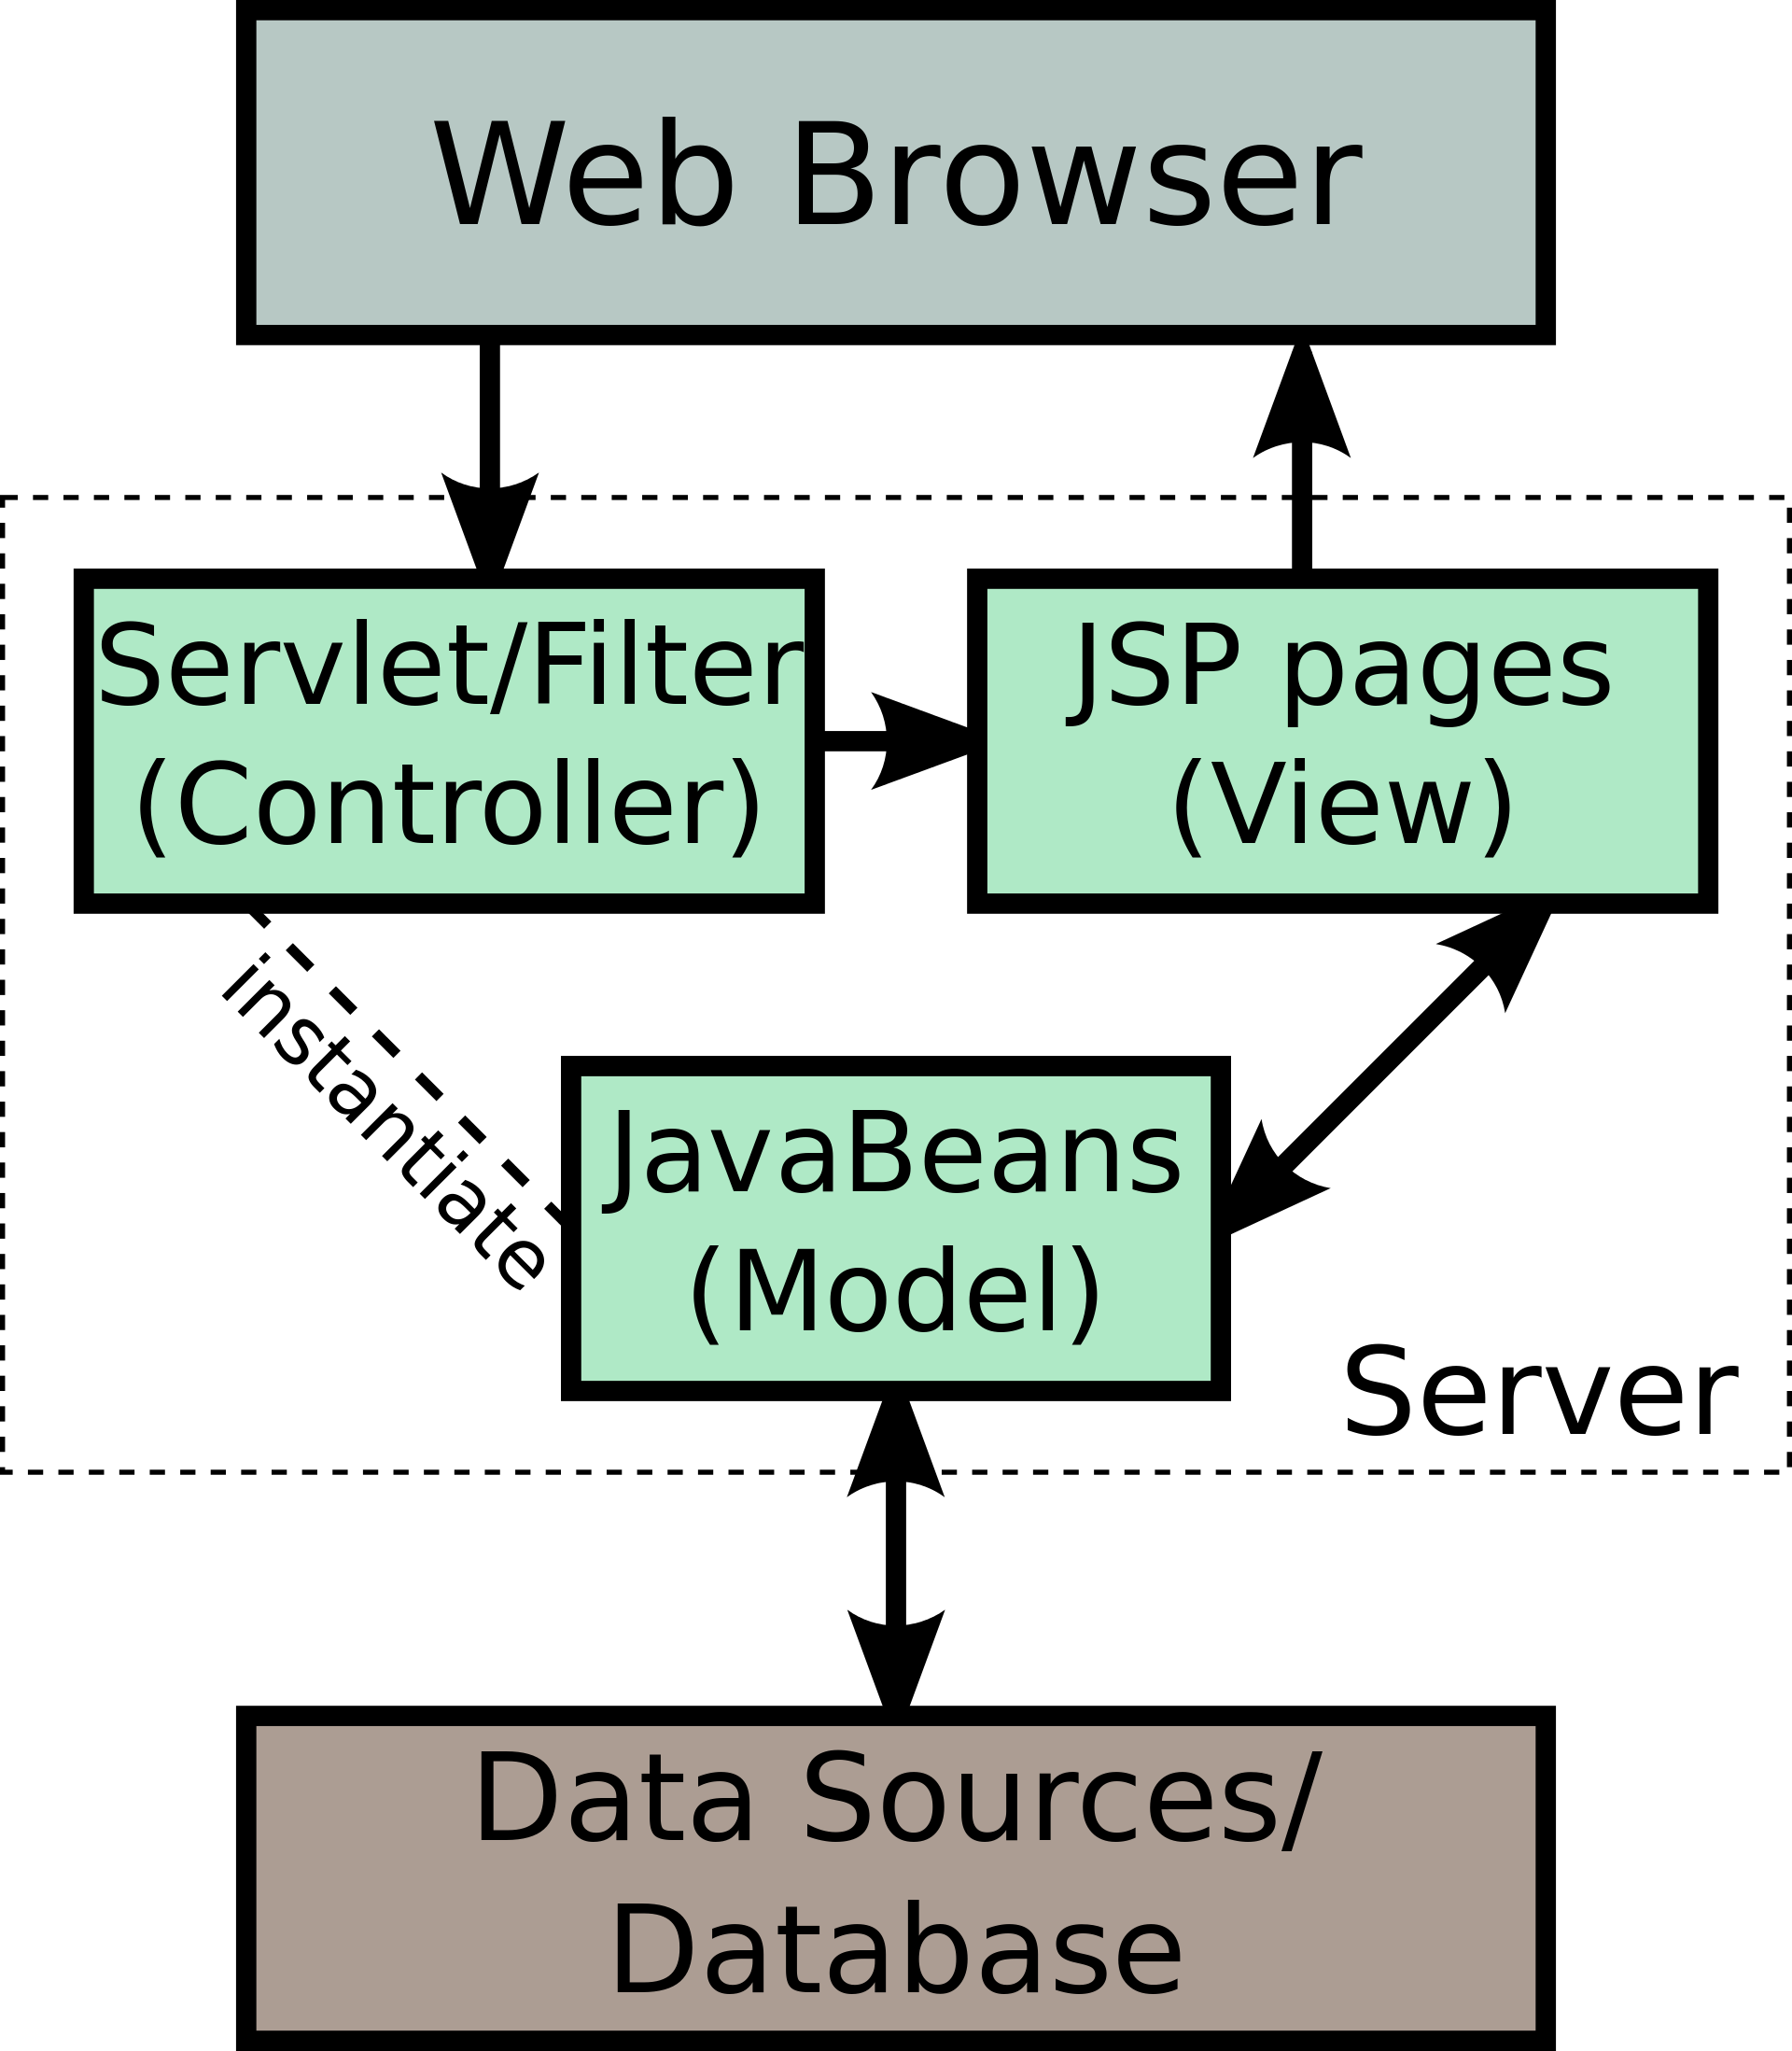
\includegraphics[width=0.4\columnwidth]{jsp_architecture}
	\caption{Esempio di interazione fra JSP, Servlet ed Enterprise JavaBeans (Fonte: \href{https://goo.gl/bWRWty}{https://goo.gl/bWRWty})}
\end{figure}

\clearpage
\section{Risultati ottenuti}
Durante tutta la durata dello stage ho prodotto i seguenti documenti:
\begin{enumerate}
	\item Ripasso dei comandi della \gls{Bash};
	\item Come funziona Hadoop e componenti principali;
	\item Funzionamento e comandi di Hive ed Impala;
	\item Funzionamento e comandi di Spark ed utilizzo in applicazioni Scala;
	\item Comandi base di Cloudera Manager;
	\item Architettura del software;
	\item Presentazione del progetto finale.
\end{enumerate}
Questa documentazione mi ha permesso di concretizzare i concetti studiati durante la prima fase e, nella successiva, di poter usufruire di una fonte di informazioni in caso di dubbi.\\\\
Per l'implementazione del prodotto ho scritto 1659 righe di codice.\\
Non ho implementato test di verifica del prodotto, come già concordato inizialmente con il tutor aziendale, in quanto il tempo a disposizione per il progetto finale era esiguo e l'interazione con l'utente era limitata alla visualizzazione di risultati e semplici richieste di elaborazione di dati.\\\\
Il bilancio del soddisfacimento dei requisiti è di seguito riportato, in cui, nella colonna "Stato", sono presenti dei codici così riepilogati:
\begin{itemize}
	\item \textcolor{green}{SO}: requisito soddisfatto;
	\item \textcolor{orange}{PS}: requisito parzialmente soddisfatto;
	\item \textcolor{red}{NS}: requisito non soddisfatto.
\end{itemize}

\clearpage
\begin{table}[!h] %
	\caption{Riepilogo soddisfacimento requisiti per la web app}
	\label{tab:soddisfacimento-app}
	\centering
	\begin{tabular}{ l | l | c}
		\textbf{Codice} & \textbf{Descrizione} & \textbf{Stato}\\
		\hline
		\hline
		\\[-2.5mm]
		RFO01 & L'utente deve poter visualizzare le statistiche \\ & delle variabili & \textcolor{green}{SO} \\
		\hline
		\\[-2.5mm]
		RFO02 & L'utente deve poter visualizzare la matrice \\ & di correlazione completa & \textcolor{green}{SO} \\
		\hline
		\\[-2.5mm]
		RFO03 & L'utente deve poter visualizzare la correlazione \\ & fra "target" e le altre variabili & \textcolor{green}{SO} \\
		\hline
		\\[-2.5mm]
		RFO04 & L'utente deve poter effettuare la ricerca di \\ & una specifica variabile & \textcolor{green}{SO} \\
		\hline
		\hline
		\\[-2.5mm]
		RFD01 & L'utente deve poter visualizzare dei grafici statistici \\ & per le variabili numeriche & \textcolor{green}{SO} \\
		\hline
		\\[-2.5mm]
		RFD02 & L'utente deve poter visualizzare dei grafici statistici \\ & per le variabili categoriali & \textcolor{green}{SO} \\
		\hline
		\\[-2.5mm]
		RFD03 & L'utente deve poter visualizzare le tre maggiori \\ & correlazioni di una variabile & \textcolor{green}{SO} \\
		\hline
		\\[-2.5mm]
		RFD04 & L'utente deve poter impostare un limite inferiore \\ & della correlazione tra "target" e le altre variabili & \textcolor{green}{SO} \\
		\hline
		\hline
		\\[-2.5mm]
		RVO01 & Utilizzo di Java EE & \textcolor{green}{SO} \\
		\hline\hline
		\\[-2.5mm]
		RVD01 & Sviluppo di un'architettura three-tier & \textcolor{green}{SO} \\
		\hline
	\end{tabular}
\end{table}%

\begin{table}[!h] %
	\caption{Bilancio soddisfacimento requisiti per la web app}
	\label{tab:bilancio-app}
	\centering
	\begin{tabular}{ c | c | c | c}
		\textbf{Importanza} & \textbf{Individuati} & \textbf{Soddisfatti} & \textbf{\%}\\
		\hline
		\hline
		\\[-2.5mm]
		Obbligatori & 5 & 5 & 100 \\
		\hline
		\\[-2.5mm]
		Desiderabili & 5 & 5 & 100 \\
		\hline
		\\[-2.5mm]
		Opzionali & 0 & 0 & 100 \\
		\hline
	\end{tabular}
\end{table}%